\section{Utilisation type}
Dans cette partie sera évoquée une description du processus de fonctionnement du programme.

\subsection{Lancement de l'application Androïd}

\paragraph{Captation d'un unique ouvrage} 


Si l'utilisateur choisit le mode de capture unique, alors le programme vérifie si l'adresse courriel est configurée ou non. 
Si elle ne l'est pas, alors le programme lance le processus de configuration. 
Une fois que celle-ci est correctement configurée, la phase de capture réelle est exécutée. 
Si l'\emph{ISBN} retourné est valide, alors le client Android envoie les informations sur le client PC. 
Si ça n'est pas le cas, il proposera à l'utilisateur de refaire une capture. 


\begin{figure}[htbp]
  \begin{center}
    \leavevmode
    \subfloat[Menu de l'application Royal\_Scanner]{%
		\label{}
		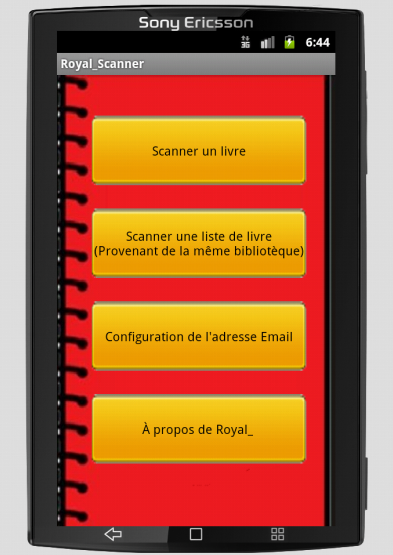
\includegraphics[height=7cm]{../img/Royal_Scanner_menu.png}}
    \hspace{4cm}
    \subfloat[Phase de capture du code-barres]{%
		\label{}
		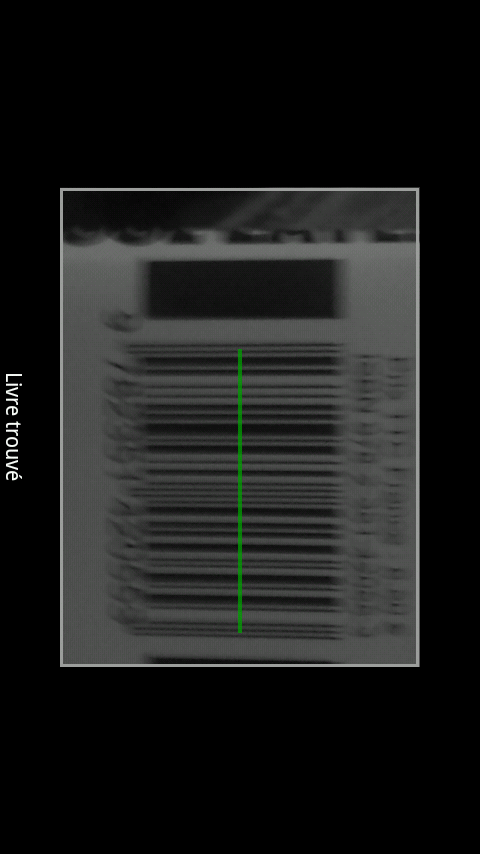
\includegraphics[height=7cm]{../img/Royal_Scanner_prisescanner_2.png}}
  \end{center}
\end{figure}

\paragraph{Capture d'un lot d'ouvrages}
Si l'utilisateur choisi de capturer directement plusieurs \emph{BDs}, alors le programme exécutera en boucle le processus utilisé pour une simple \emph{BD}. 
Le seul changement interviendra après la validation de la bonne capture de l'\emph{ISBN} :
Il sera en effet demandé à l'utilisateur si celui-ci désire continuer la capture ou d'y mettre fin. 

S'il choisit d'y mettre fin, alors les informations seront transmises au client PC. 
Si au contraire, il choisit de continuer la capture, alors le programme rebouclera. 

\subsection{Lancement de l'application PC}


\begin{wrapfigure}[5]{r}[1cm]{5cm}
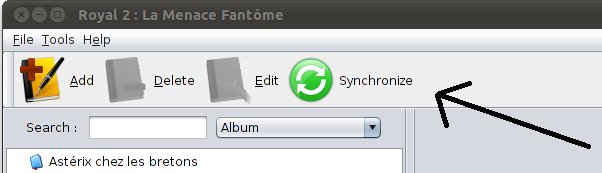
\includegraphics[width=5cm]{../img/btn_synchro.png}
\caption{Bouton d'importation}
\end{wrapfigure}
\paragraph{Importation des livres}
Si l'utilisateur choisit d'importer les livres. Alors, le programme teste si l'adresse courriel est correctement configurée. Si ce n'est pas le cas, le processus de configuration est exécuté. 

Une fois que le programme a une configuration de courriel valide, celui-ci y recherche les messages présents à son attention. 

\begin{wrapfigure}[12]{r}[1.5cm]{8cm}
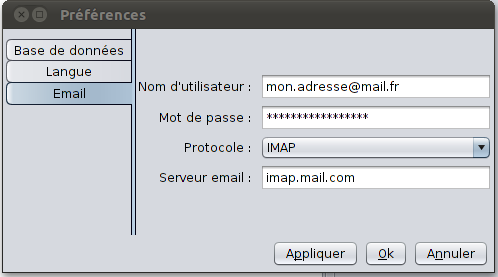
\includegraphics[width=8cm]{../img/preferenceMail.png}
\caption{Configuration du mail}
\end{wrapfigure}
\paragraph{Importation des livres}
Tant qu'il y a des messages à l'attention du programme, celui-ci les lit. 
Tant que des numéros d'\emph{ISBN} sont présents dans le courriel, ils sont récupérés. 
Une fois tous les \emph{ISBN} récupérés, le programme recherche des informations sur les livres sur internet.
L'utilisateur peut ensuite modifier ces données, puis peut renseigner les informations relatives à la bibliothèque. 

Si la bibliothèque dans là quelle le livre (ou le lot) a été emprunté existe déjà, 
alors l'utilisateur n'aura qu'à la choisir dans une liste. Si elle n'existe pas encore, elle pourra être rajoutée via une fonction disponible. 
Enfin, l'utilisateur pourra indiquer la date de retour maximale du livre (ou du lot).

\paragraph{Vérification de la date de retour}
À chaque lancement de programme, les dates de tous les ouvrages encore en possession de l'utilisateur seront testées afin de voir si l'ultimatum n'est pas arrivé à terme. 
Les noms de tous les livres ainsi repérés sont conservés puis affichés à l'utilisateur une fois la recherche terminée. 


\begin{wrapfigure}[12]{l}[1cm]{8cm}
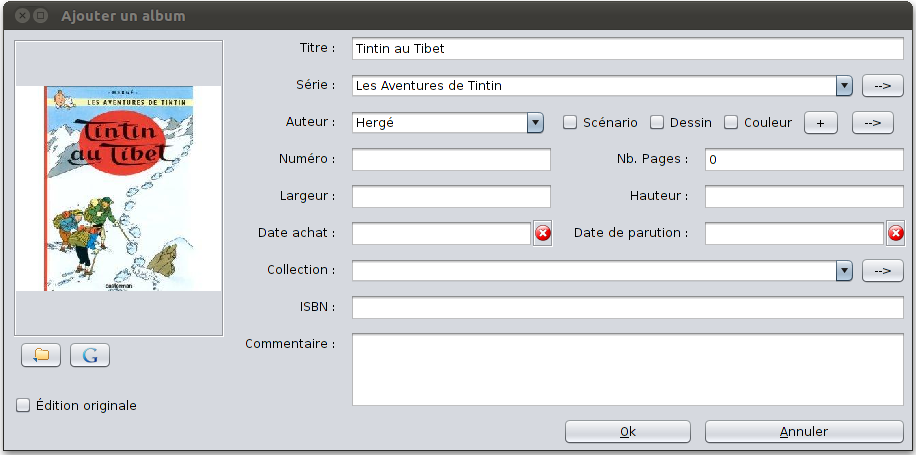
\includegraphics[width=8cm]{../img/editionAlbum.png}
\caption{Edition d'un Album}
\end{wrapfigure}

\paragraph{Modification des informations d'un livre}
Si l'utilisateur souhaite modifier des informations sur un livre enregistré dans le programme, il pourra visualiser les albums par critères tels que l'auteur, la collection, le type…
Une fois le livre sélectionné, il faudra cliquer sur le bouton « éditer ».  
C'est à ce moment que l'utilisateur verra apparaitre les différentes informations sur le livre et pourra les modifier.
Une fois satisfait des changements, l'utilisateur pourra soit valider les modifications, soit les annuler. 
En cas de validation de la modification, le programme enregistrera les nouvelles informations dans la base de données.  
